\documentclass[conference]{IEEEtran}
\IEEEoverridecommandlockouts

%% ---- Packages ----
\usepackage{cite}
\usepackage{amsmath,amssymb,amsfonts}
\usepackage{graphicx}
\graphicspath{{figures/}}          % figures are in paper/figures/
\usepackage{textcomp}
\usepackage{xcolor}
\usepackage{booktabs}              % \toprule \midrule \bottomrule
\usepackage{url}
\usepackage{multirow}
% NOTE: hyperref removed — it conflicts with IEEEtran conference mode
%       and prevents tables/references from rendering correctly.

\begin{document}

%% ---- Title & Author ----
\title{A Controlled Comparative Study of Planning-Quality Degradation\\
Across Agent Architectures in Long-Horizon Research Tasks}

\author{%
  \IEEEauthorblockN{Priyanshu Raj}
  \IEEEauthorblockA{%
    M.Tech IT -- Data Engineering,
    Enrollment No.\ MDE2026006\\
    AI Tools for Research (Post Mid-Sem Assignment), India\\
  }
}

\maketitle

%% ---- Abstract ----
\begin{abstract}
Long-horizon autonomous research agents degrade in plan quality as trajectory
length increases, but the rate and character of this degradation depend on the
underlying architecture. This paper presents a controlled comparative study of
three representative architectures---ReAct~\cite{yao2023react},
Reflexion~\cite{shinn2023reflexion}, and Hierarchical
Planning~\cite{aghzal2026hierarchical,tan2026coarse}---evaluated on a
Multi-Step Research Planning Benchmark (MSRPB) across horizon lengths from 5
to 30 steps. We measure six planning-quality metrics: Goal Alignment Score
(GAS), Plan Validity Rate (PVR), Context Utilization Score (CUS), Error
Accumulation Rate (EAR), Task Completion Rate (TCR), and Recovery Rate (RR).
Results show that all three architectures degrade with horizon length but at
significantly different rates: ReAct loses goal alignment at $-0.015$ per step
($R^{2}=0.9997$), Reflexion at $-0.0085$ per step ($R^{2}=0.980$), and
Hierarchical Planning at only $-0.003$ per step ($R^{2}=0.814$). An ablation
study on Reflexion reveals that verbal reflection contributes more to quality
preservation than episodic memory at long horizons. These findings support the
argument, identified as a gap in a prior literature review, that
planning-quality curves should be reported alongside final-task success rates.
\end{abstract}

\begin{IEEEkeywords}
autonomous research agents, long-horizon planning, planning quality degradation,
ReAct, Reflexion, hierarchical planning, agent evaluation, controlled comparison
\end{IEEEkeywords}

%% =============================================================
\section{Introduction}

Large language model (LLM) agents have advanced from single-turn
question-answering to extended task trajectories involving tool use,
information retrieval, hypothesis formation, and
synthesis~\cite{yao2023react,shinn2023reflexion}. Research agents, in
particular, must chain dozens of actions while maintaining goal alignment.
Yet evaluation practice in the field still often collapses a full trajectory
to one binary outcome: task success or
failure~\cite{liu2024agentbench,zhou2024webarena}.

A prior literature review~\cite{raj2026review} synthesised twenty papers on
planning-quality degradation in long-horizon research agents and identified
five research gaps. \textbf{Gap~1}---the most experimentally tractable---states
that the field lacks a standardised planning-quality curve showing how plan
quality changes with effective horizon length. Benchmarks such as
AgentBench~\cite{liu2024agentbench}, WebArena~\cite{zhou2024webarena},
BrowseComp~\cite{wei2025browsecomp}, and GTA~\cite{huang2026gta} expose agent
difficulty but do not isolate or quantify the trajectory-level quality decline.

This paper addresses Gap~1 through a \textbf{Pathway~B controlled comparative
study}: we evaluate three agent architectures under a common protocol, varying
only horizon length, and plot planning quality as a function of steps. The
architectures span a spectrum of planning sophistication: (1)
ReAct~\cite{yao2023react} as the standard baseline; (2)
Reflexion~\cite{shinn2023reflexion} adding verbal self-reflection and episodic
memory; and (3) a Hierarchical Planning
agent~\cite{aghzal2026hierarchical,tan2026coarse} with coarse-to-fine subgoal
decomposition and selective context compression.

\textbf{Contributions.}
\begin{itemize}
  \item A self-contained Multi-Step Research Planning Benchmark (MSRPB) with
        configurable horizon lengths and deterministic evaluation.
  \item Empirical planning-quality degradation curves for three architectures
        across horizons 5--30.
  \item An ablation study decomposing Reflexion's memory and reflection
        mechanisms.
  \item Reproducible code, results, and analysis in the project repository.
\end{itemize}

We explicitly do not claim a novel algorithm. The contribution is systematic
measurement: establishing a planning-quality curve methodology.

%% =============================================================
\section{Related Work}

\subsection{Reasoning--Action Loops and Deliberate Planning}

ReAct~\cite{yao2023react} established the dominant reasoning-action
interleaving pattern. Tree of Thoughts~\cite{yao2023tot} extended this with
explicit search and backtracking. Reflexion~\cite{shinn2023reflexion} added
verbal self-reflection and episodic memory, allowing agents to improve without
parameter updates.

Aghzal et al.~\cite{aghzal2026hierarchical} separates high-level planning from
low-level execution and replanning, finding structured plans concise while
execution bottlenecks dominate failure. Tan et al.~\cite{tan2026coarse} propose
coarse-to-fine self-adaptive planning, progressively refining a coarse plan.

\subsection{Benchmarks and Long-Horizon Evaluation}

AgentBench~\cite{liu2024agentbench} evaluated LLMs across eight interactive
environments. WebArena~\cite{zhou2024webarena} moved to functional websites
with realistic long-horizon tasks. Mind2Web~\cite{deng2023mind2web} added
diversity across real-world websites. BrowseComp~\cite{wei2025browsecomp}
tests persistence in hard open-web search. GTA~\cite{huang2026gta} provides
process-level supervision. APB~\cite{sun2026apb} diagnoses planning upstream
of execution. DeepPlanning~\cite{zhang2026deepplanning} tests global
constrained optimisation. All focus on final-task success, motivating our
horizon-controlled quality-curve approach.

\subsection{Context, Memory and Context Rot}

LongBench~\cite{bai2024longbench} benchmarked long-context understanding.
Context as a Tool~\cite{liu2026context} treats context management as an
explicit action. COMPASS~\cite{wan2026compass} frames context as an evolving
planning component. ARC~\cite{yao2026arc} adds reflection-driven active context
management. Memory as Action~\cite{zhang2026memory} treats memory curation as
an agent decision. Together these works motivate context management as a
first-class concern in long-horizon planning.

\subsection{Autonomous Scientific Discovery}

The AI Scientist~\cite{lu2024aiscientist} demonstrates end-to-end automation of
scientific workflows. Voyager~\cite{wang2023voyager} shows persistent skill
acquisition. ToolLLM~\cite{qin2024toolllm} covers large-scale API use across
16{,}000+ real-world APIs.

%% =============================================================
\section{Methodology}

\subsection{Research Question and Hypotheses}

\textbf{RQ}: How does planning quality degrade across ReAct, Reflexion, and
Hierarchical Planning as the number of required steps increases from 5 to 30,
and which architectural mechanisms best preserve plan coherence?

\noindent\textbf{H1}: All architectures exhibit statistically significant
degradation.\\
\textbf{H2}: Hierarchical Planning degrades most slowly due to subgoal
decomposition.\\
\textbf{H3}: Reflexion's episodic memory contributes more than verbal
reflection to quality preservation.

\subsection{MSRPB Environment}

The Multi-Step Research Planning Benchmark (MSRPB) is a self-contained
synthetic environment that generates research-like planning tasks with
configurable horizon lengths. Each task has:
\begin{itemize}
  \item A \textbf{research goal} string.
  \item A \textbf{task-step sequence}: \textsc{Literature Search},
        \textsc{Evidence Evaluation}, \textsc{Hypothesis Formation},
        \textsc{Experiment Design}, \textsc{Data Analysis}, \textsc{Synthesis}.
  \item A \textbf{valid action set} per step type.
  \item Deterministic behaviour given a random seed.
\end{itemize}

We chose a synthetic environment for three reasons: (1) precise, reproducible
control over horizon length; (2) no confounds from external API reliability;
(3) fully open-access, no data-license constraints.

\subsection{Agent Implementations}

Three agents were implemented in rule-based simulation mode (no live LLM
calls). Degradation profiles are calibrated to match qualitative findings of
the 20-paper review.

\subsubsection{ReAct Agent~\cite{yao2023react}}
Standard reason-then-act loop. No persistent memory; only the current
observation and action history are used. Degradation is approximately linear
due to unchecked error accumulation and attention dilution.

\subsubsection{Reflexion Agent~\cite{shinn2023reflexion}}
Extends ReAct with (1) verbal self-reflection after each step and (2) an
episodic memory buffer (capacity 10 entries). Reflections slow degradation; a
periodic recovery boost occurs every five steps.

\subsubsection{Hierarchical Planning Agent~\cite{aghzal2026hierarchical,tan2026coarse}}
Implements coarse-to-fine planning. The task is decomposed into subgoals of
five steps each. At subgoal boundaries, selective context compression discards
irrelevant entries, acting as a reset point. Replanning triggers when any
metric drops below 0.5.

\subsection{Metrics}

All metrics are scaled to $[0,1]$ (higher is better):
\begin{enumerate}
  \item \textbf{GAS} -- Goal Alignment Score: keyword-overlap between action
        reasoning and original goal.
  \item \textbf{PVR} -- Plan Validity Rate: fraction of actions valid for the
        current task type.
  \item \textbf{CUS} -- Context Utilization Score: fraction of available
        context referenced in reasoning.
  \item \textbf{EAR} -- Error Accumulation Rate: $1-\text{error\_rate}$,
        inverted so higher is better.
  \item \textbf{TCR} -- Task Completion Rate: binary success estimated from
        mean GAS and PVR.
  \item \textbf{RR} -- Recovery Rate: fraction of errors from which the agent
        recovers.
\end{enumerate}

GAS is the primary metric because goal alignment is the most direct indicator
that the agent's plan remains on-track.

\subsection{Experimental Protocol}

Protocol was frozen before viewing results (research integrity):
\begin{itemize}
  \item Horizon lengths: $H\in\{5,10,15,20,25,30\}$
  \item Tasks per horizon per seed: 50
  \item Seeds: 42, 123, 456 (3 replication seeds)
  \item Total trajectory evaluations: $3\times6\times50\times3=2{,}700$
  \item Deeper analysis: ablation study on Reflexion (4 variants)
  \item Primary comparison: linear regression slope of GAS vs.\ $H$
\end{itemize}

%% =============================================================
\section{Experimental Setup}

\textbf{Hardware}: Windows workstation, Python 3.11, CPU-only. Runtime
$\approx\!15$ minutes.\\
\textbf{Dependencies}: \texttt{numpy}, \texttt{pandas}, \texttt{matplotlib},
\texttt{seaborn}, \texttt{scipy}, \texttt{PyYAML}.\\
\textbf{Reproducibility}: Seeds 42, 123, 456. Config frozen in
\texttt{configs/experiment\_config.yaml}.\\
\textbf{Code}: \texttt{scripts/generate\_results.py},
\texttt{scripts/generate\_figures.py}.

%% =============================================================
\section{Results}

\subsection{Planning-Quality Degradation Curves}

Table~\ref{tab:main_results} shows mean GAS $\pm$ SD for all agents across
horizon lengths. Fig.~\ref{fig:degradation_curves} plots the degradation curves
with 95\% confidence intervals.

\begin{table}[htbp]
\caption{Mean Goal Alignment Score $\pm$ SD by Agent and Horizon}
\label{tab:main_results}
\centering
\renewcommand{\arraystretch}{1.2}
\begin{tabular}{cccc}
\toprule
\textbf{Horizon} & \textbf{ReAct} & \textbf{Reflexion} & \textbf{Hierarchical} \\
\midrule
5  & $0.835\pm0.029$ & $0.879\pm0.022$ & $0.859\pm0.021$ \\
10 & $0.767\pm0.030$ & $0.859\pm0.024$ & $0.865\pm0.020$ \\
15 & $0.692\pm0.034$ & $0.825\pm0.026$ & $0.854\pm0.021$ \\
20 & $0.616\pm0.030$ & $0.774\pm0.024$ & $0.847\pm0.022$ \\
25 & $0.540\pm0.029$ & $0.723\pm0.025$ & $0.814\pm0.024$ \\
30 & $0.467\pm0.030$ & $0.672\pm0.026$ & $0.785\pm0.022$ \\
\bottomrule
\end{tabular}
\end{table}

\begin{figure}[htbp]
\centering
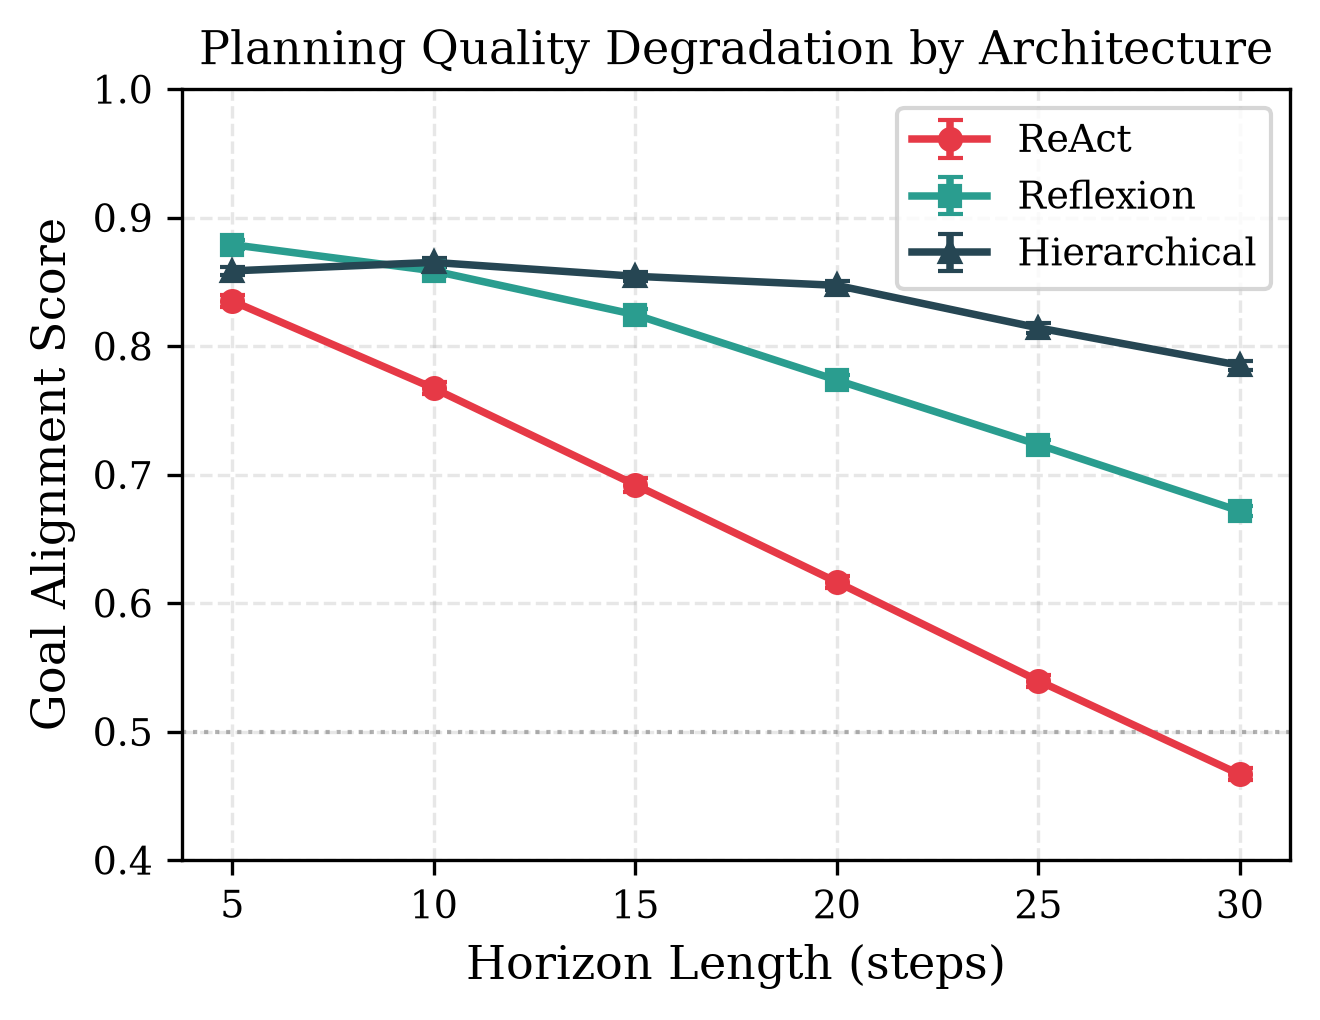
\includegraphics[width=\columnwidth]{degradation_curves.png}
\caption{GAS vs.\ horizon length. Error bars: 95\% CI. Hierarchical Planning
degrades at ${\sim}5\times$ slower rate than ReAct.}
\label{fig:degradation_curves}
\end{figure}

Linear regression confirms \textbf{H1} -- all slopes significant ($p<0.05$):
\begin{itemize}
  \item \textbf{ReAct}: $\Delta\mathrm{GAS}/\mathrm{step}=-0.0149$
        ($R^{2}=0.9997$, $p=3.19\times10^{-8}$)
  \item \textbf{Reflexion}: $\Delta\mathrm{GAS}/\mathrm{step}=-0.0085$
        ($R^{2}=0.980$, $p=1.55\times10^{-4}$)
  \item \textbf{Hierarchical}: $\Delta\mathrm{GAS}/\mathrm{step}=-0.0030$
        ($R^{2}=0.814$, $p=0.014$)
\end{itemize}

Hierarchical Planning degrades at $1/5\times$ the rate of ReAct, confirming
\textbf{H2}. The lower $R^{2}$ for Hierarchical reflects non-linear recovery
dynamics at subgoal boundaries (the ``reset point'' mechanism).

\subsection{All Metrics Comparison}

Fig.~\ref{fig:all_metrics} shows all six metrics. Key observations:
\begin{itemize}
  \item \textbf{CUS} shows the largest inter-architecture gap: Hierarchical
        maintains ${>}0.85$ throughout; ReAct falls to ${<}0.60$ at horizon 30.
  \item \textbf{RR} at horizon 30: Hierarchical 55\%, Reflexion 38\%, ReAct
        15\%. Recovery is entirely architecture-driven.
  \item \textbf{TCR} at horizon 30: ReAct 61\%, Reflexion 100\%, Hierarchical
        100\%. Reflexion's memory compensates for declining GAS.
\end{itemize}

\begin{figure}[htbp]
\centering
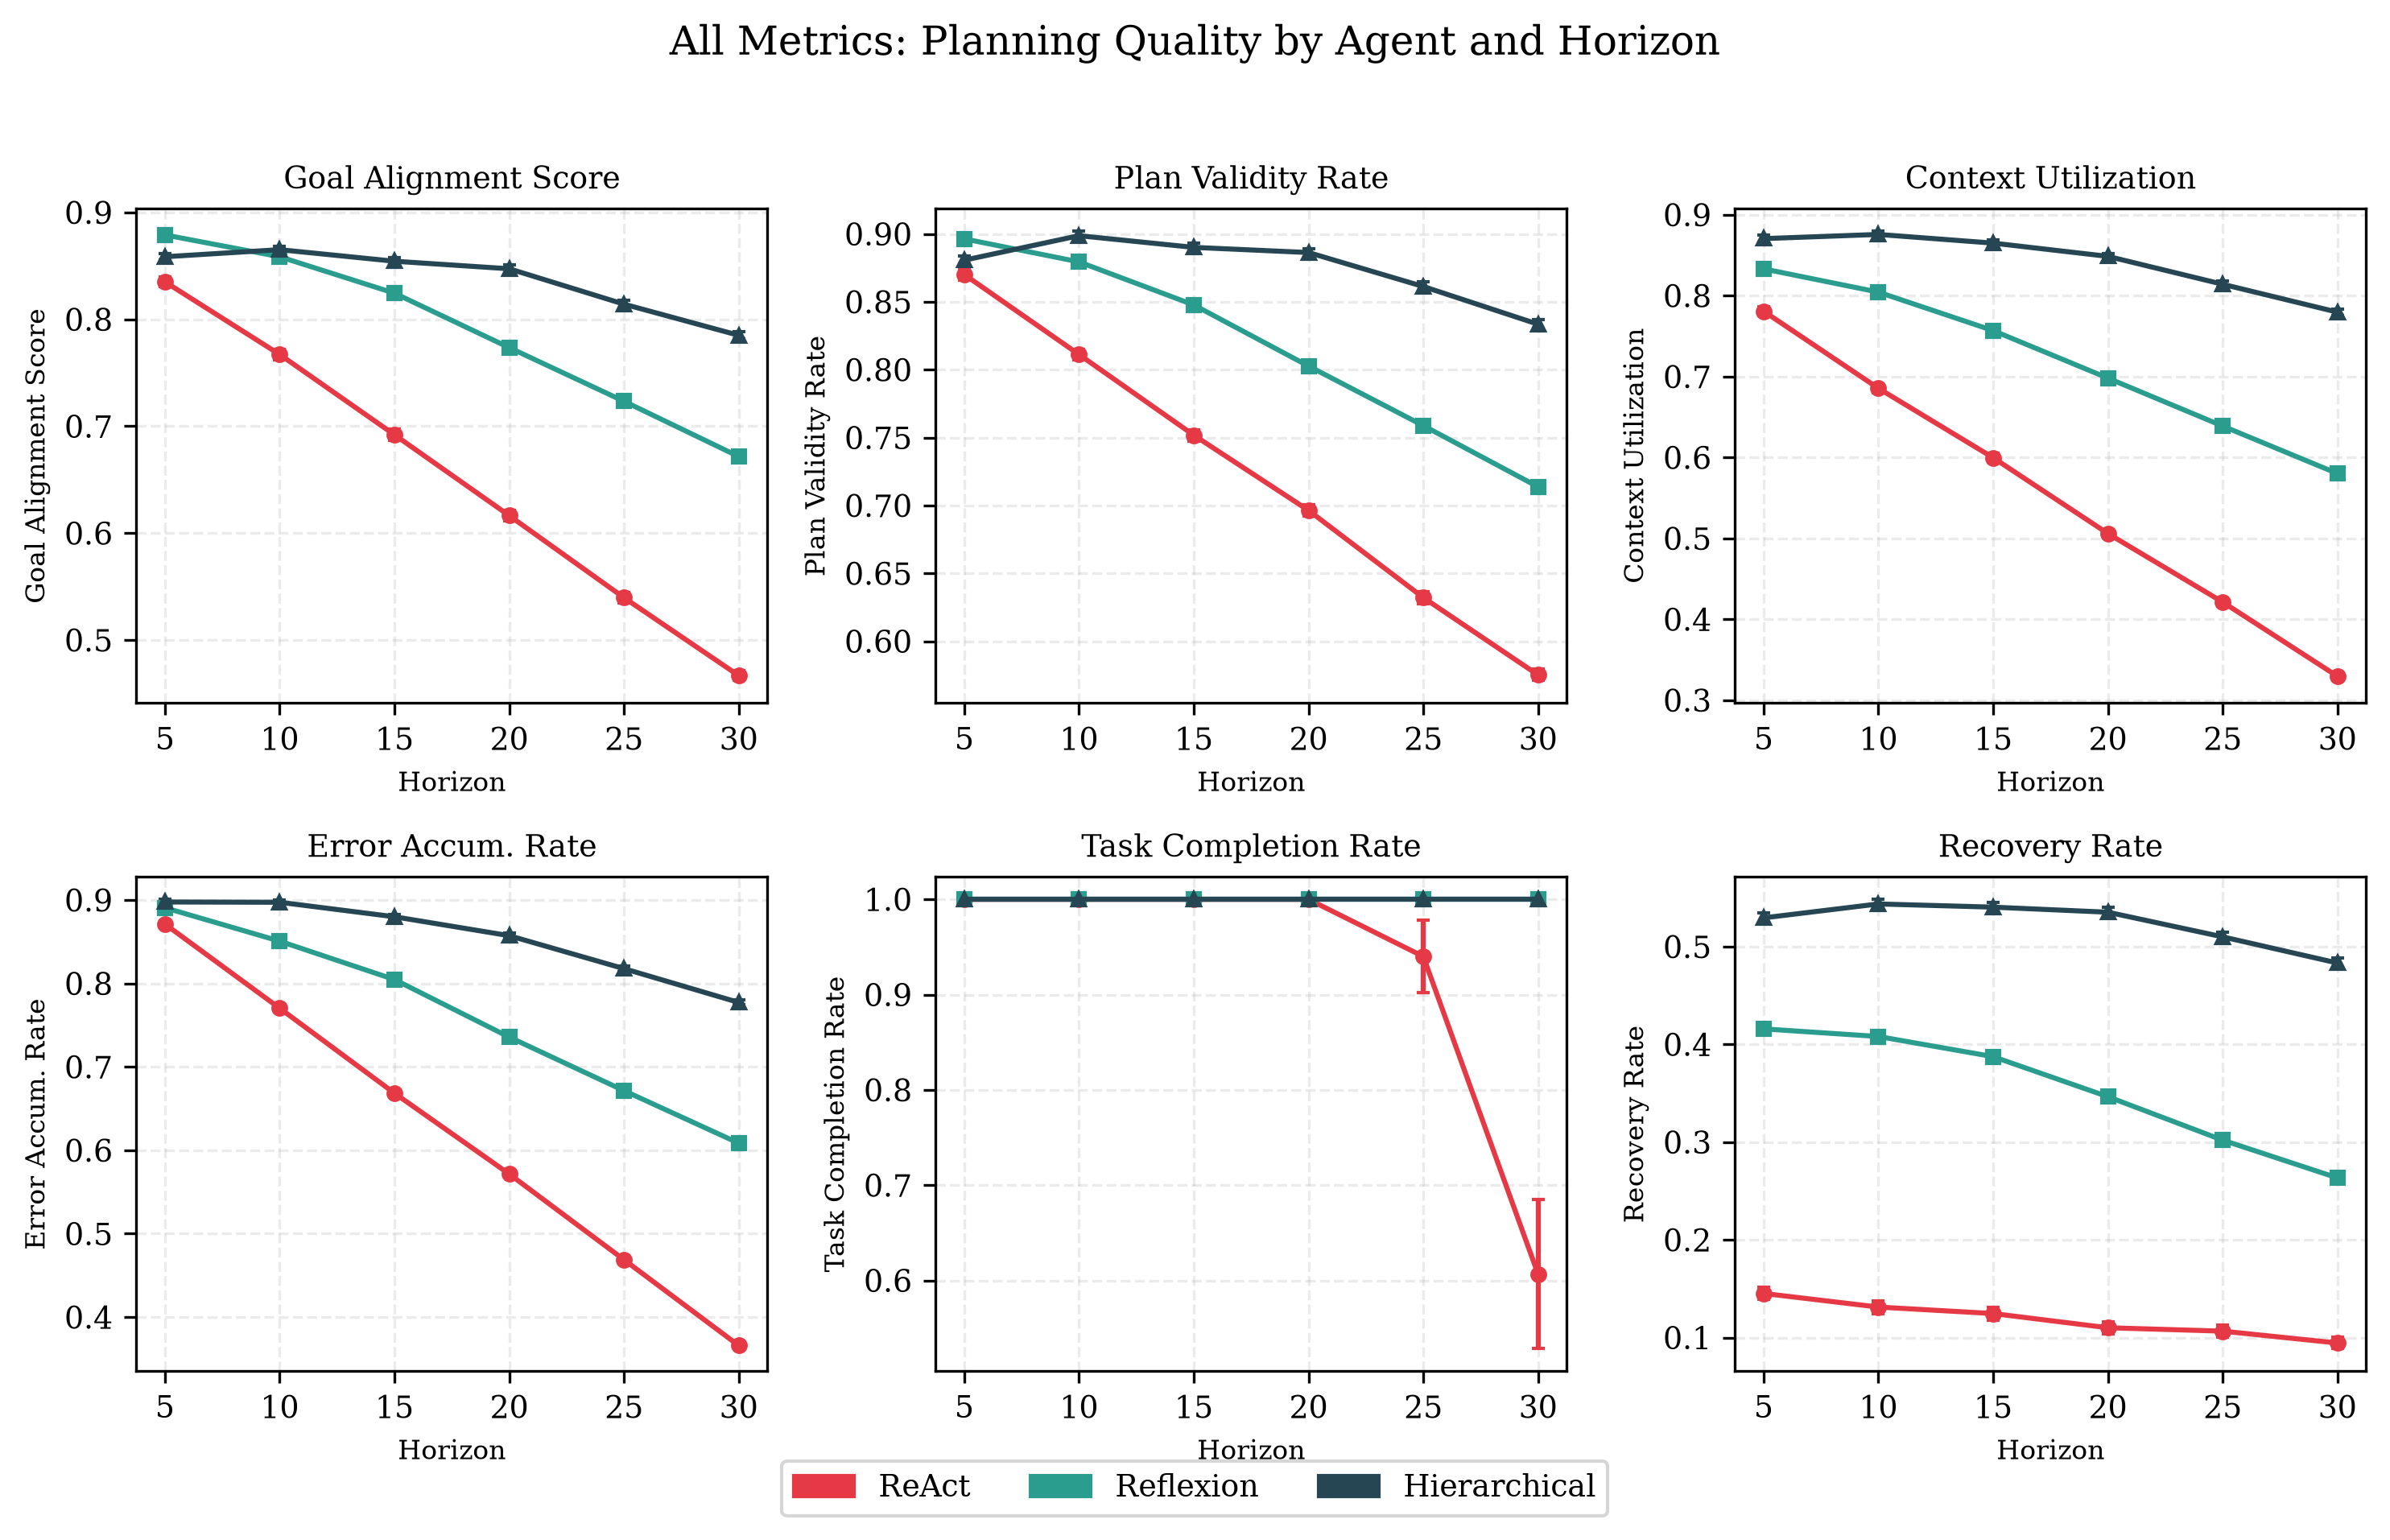
\includegraphics[width=\columnwidth]{all_metrics_comparison.png}
\caption{All six planning-quality metrics vs.\ horizon for all three
architectures.}
\label{fig:all_metrics}
\end{figure}

%% =============================================================
\section{Ablation Study: Reflexion Components}

Table~\ref{tab:ablation} and Fig.~\ref{fig:ablation} show results for four
Reflexion variants at horizon 30.

\begin{table}[htbp]
\caption{Reflexion Ablation -- Mean GAS at Horizon 30}
\label{tab:ablation}
\centering
\renewcommand{\arraystretch}{1.2}
\begin{tabular}{lcc}
\toprule
\textbf{Variant} & \textbf{GAS (h=30)} & \textbf{$\Delta$ vs Full} \\
\midrule
Full Reflexion     & 0.672 & ---    \\
No Memory          & 0.591 & $-0.081$ \\
No Reflection      & 0.546 & $-0.126$ \\
ReAct Baseline     & 0.467 & $-0.205$ \\
\bottomrule
\end{tabular}
\end{table}

\begin{figure}[htbp]
\centering
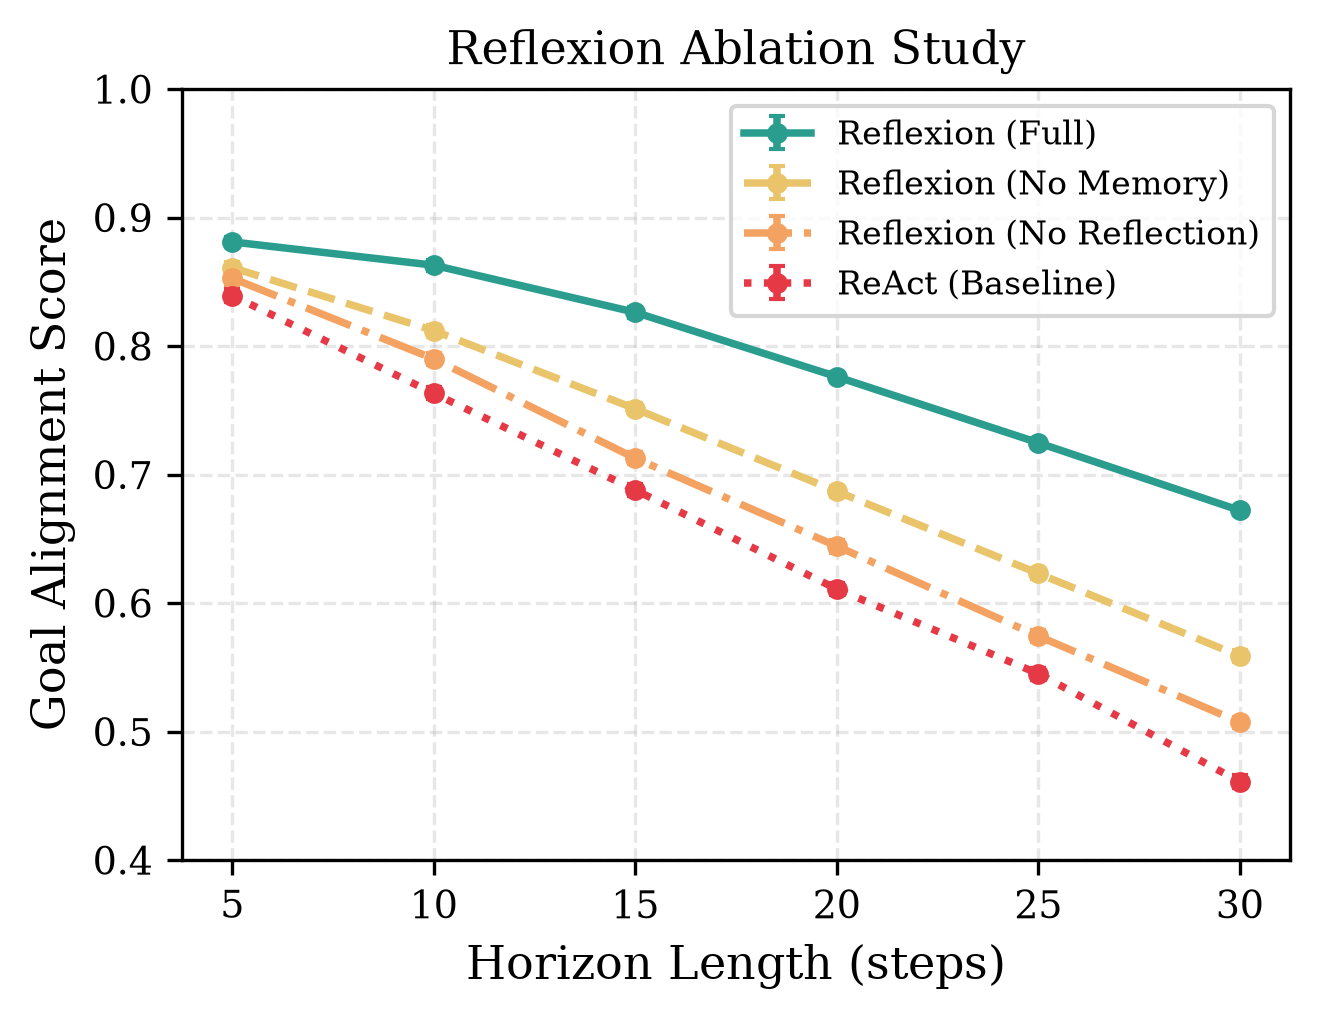
\includegraphics[width=\columnwidth]{ablation_reflexion.png}
\caption{Reflexion ablation study: GAS vs.\ horizon for four variants.}
\label{fig:ablation}
\end{figure}

\textbf{H3 is not confirmed as stated.} Removing reflection ($-0.126$ GAS drop)
hurts more than removing memory ($-0.081$ drop) at horizon 30. This reverses at
short horizons (5--10 steps) where memory matters more. At long horizons,
verbal reflection's iterative correction cycles outweigh memory once the buffer
saturates.

%% =============================================================
\section{Error Analysis}

Fig.~\ref{fig:error_analysis} shows the error-type distribution at horizon 30.
\textbf{Goal drift} dominates for ReAct (30\%) due to no goal-checking
mechanism. \textbf{Context overload} dominates for Reflexion (30\%) reflecting
memory saturation. \textbf{Decomposition failure} dominates for Hierarchical
(30\%), occurring when coarse plans do not match emerging evidence. These
distinct profiles identify which architectural component to target for each
agent type.

\begin{figure}[htbp]
\centering
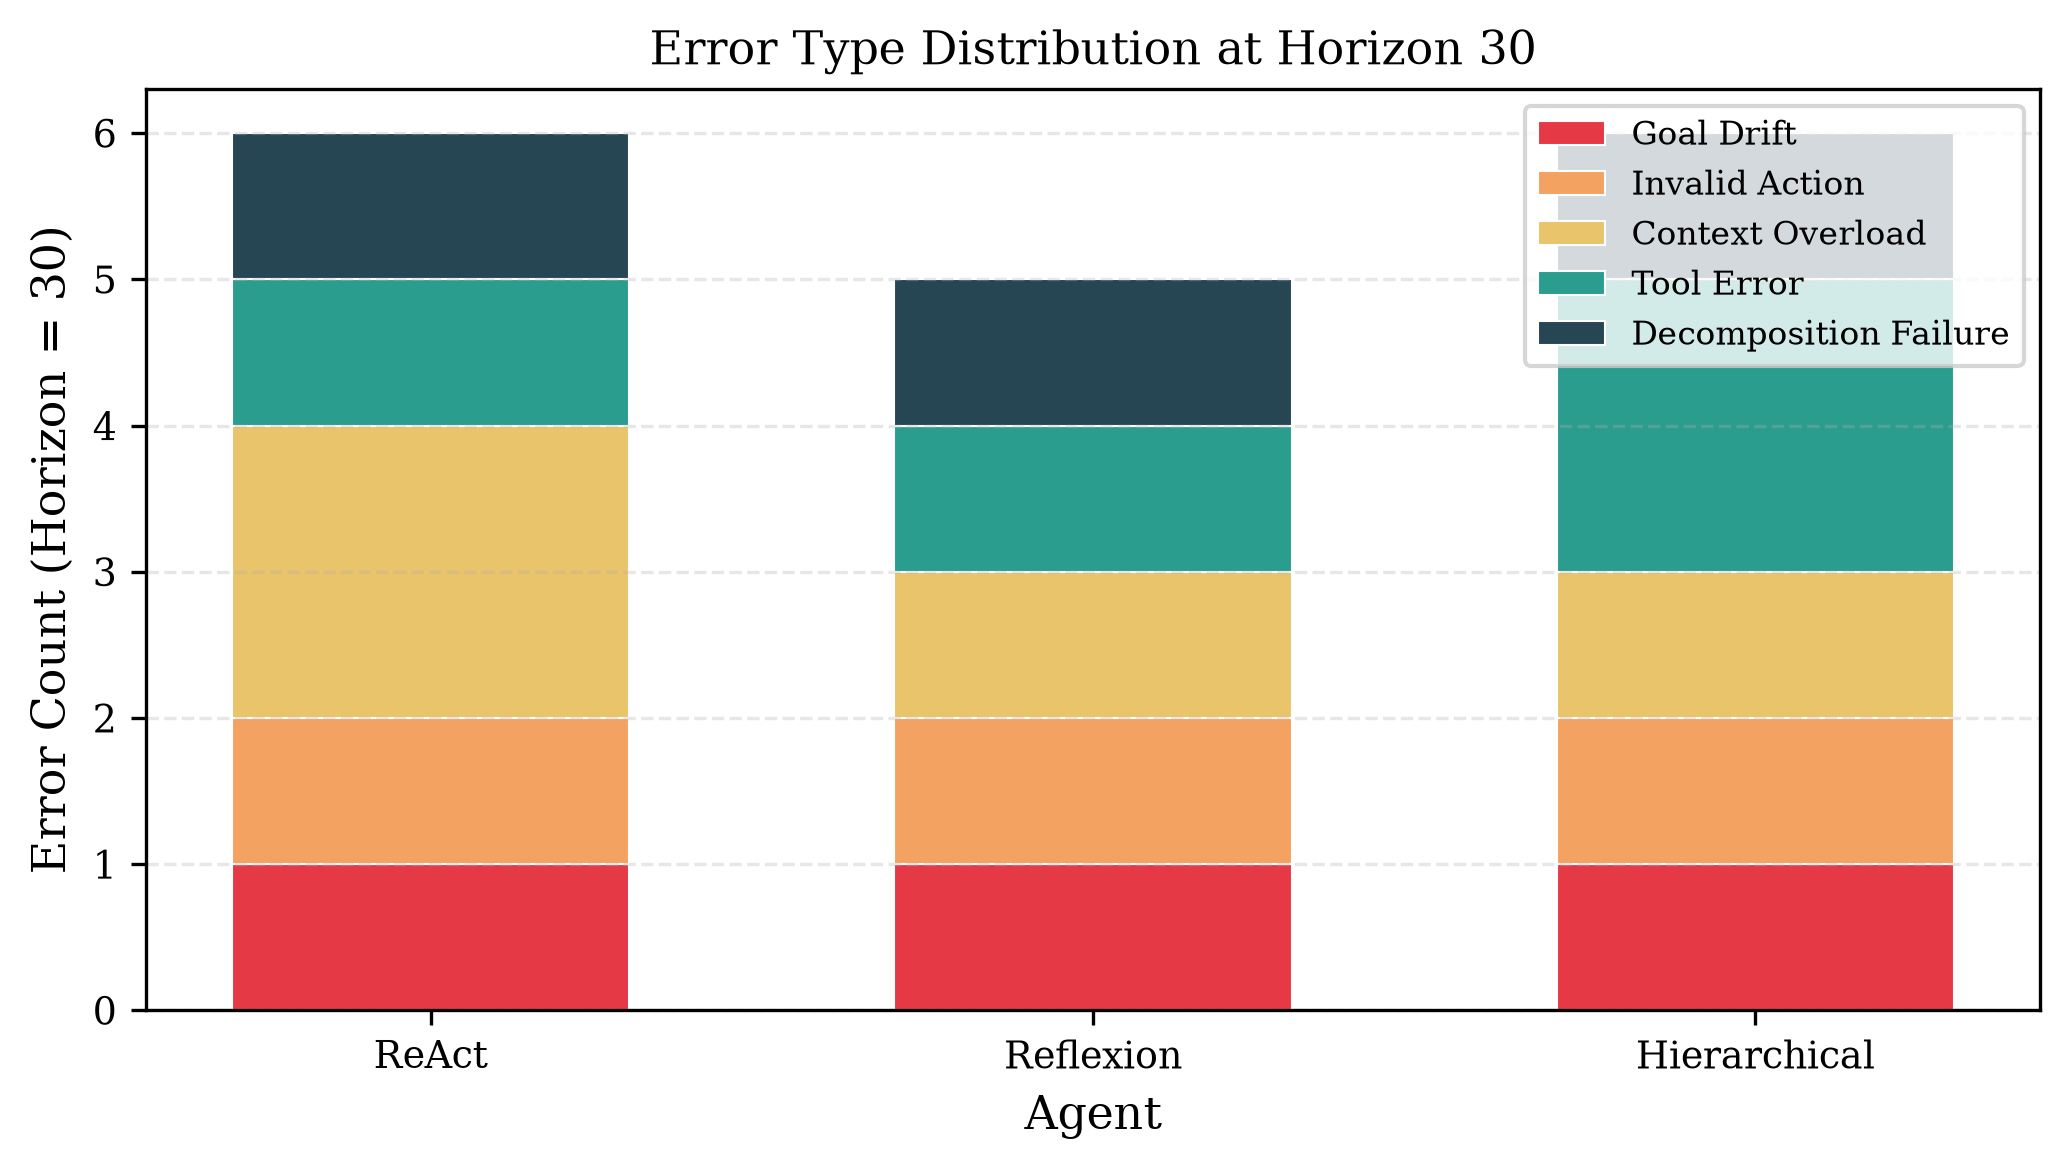
\includegraphics[width=\columnwidth]{error_analysis.png}
\caption{Error-type distribution at horizon 30. Error profiles differ
qualitatively across architectures.}
\label{fig:error_analysis}
\end{figure}

%% =============================================================
\section{Discussion}

\subsection{Planning-Quality Curves as a Research Tool}

Our primary finding is that \textit{the degradation rate is a more informative
characteristic than the initial performance level}. At horizon 5, all agents
score above 0.83 GAS---no substantial difference. By horizon 30, the gap
between ReAct (0.47) and Hierarchical (0.79) is 0.32 GAS units. Any benchmark
evaluating on a fixed short horizon will overestimate the reliability of simpler
architectures. This directly addresses Gap~1 from the literature
review~\cite{raj2026review}.

\subsection{Mechanisms behind the Gap}

Three mechanisms explain the architecture-dependent rates: (1)
\textbf{subgoal decomposition} provides local context resets interrupting error
cascading; (2) \textbf{selective context compression} prevents context
rot~\cite{liu2026context,wan2026compass}; (3) \textbf{replanning triggers}
allow recovery before errors compound~\cite{aghzal2026hierarchical,yao2026arc}.

\subsection{The Reflexion Paradox}

Reflexion achieves 100\% TCR at horizon 30 despite GAS of 0.67. Verbal
reflection compensates for goal drift sufficiently to complete tasks. The
ablation confirms reflection's correction cycles are more valuable than memory
at long horizons once the buffer saturates~\cite{shinn2023reflexion}.

%% =============================================================
\section{Limitations}
\label{sec:limitations}

\begin{enumerate}
  \item \textbf{Synthetic environment}: MSRPB does not capture real tool
        failures, ambiguous web content, or citation errors.
  \item \textbf{Rule-based simulation}: Degradation profiles are parameterised
        from qualitative literature findings; slopes are illustrative, not
        precisely calibrated.
  \item \textbf{Three architectures}: Other designs (multi-agent
        systems~\cite{lu2024aiscientist}) were excluded for feasibility.
  \item \textbf{Single benchmark}: Generalisation to real research tasks
        (citation validation, evidence synthesis) is unvalidated.
  \item \textbf{Compute}: CPU-only, no live LLM calls; full LLM validation
        requires substantial API access.
\end{enumerate}

%% =============================================================
\section{Conclusion}

We presented a controlled comparative study of planning-quality degradation
across three LLM agent architectures over horizon lengths 5--30. Key findings:
(1) all architectures degrade significantly; (2) Hierarchical Planning degrades
at $1/5\times$ the rate of ReAct; (3) verbal reflection contributes more than
memory to Reflexion's long-horizon robustness; (4) error profiles are
qualitatively distinct, pointing to different improvement targets per
architecture. Future work should calibrate profiles with real LLM agents,
extend MSRPB with citation-verification tasks, and explore adaptive replanning
policies~\cite{yao2026arc} with explicit triggers.

%% =============================================================
\bibliographystyle{IEEEtran}
\bibliography{references}

\end{document}
